\subsection{Implementierung von Unit-Tests (Modelltests)}    
\label{sec:awunit}

Ein Rails-Modell, wie in \ref{sec:railsconcepts} auf S. \pageref{sec:railsconcepts} beschrieben, repräsentiert die Daten der Anwendung, und die Regeln, wie diese zu verändern sind. Bei Rails werden sie hauptsächlich dazu verwendet, um mit der zugrundeliegenden Datenbanktabelle zu interagieren. Per Konvention von Rails findet hier die Hauptarbeit, also die Business-Logik, statt.

Fast jeder Unittest bei Rails beinhaltet das Testen auf Validierungskritieren seines korrespondierenden Modells, d.h. wann eine Instanz dieses Modells gültig ist und damit gespeichert werden darf (man denke z.B. an Pflichtfelder für ein Modell "`Nutzer"` oder die Validierung des Formates seiner E-Mail-Adresse). Weiterhin sollten natürlich alle weiteren, selbstdefinierten, Methoden getestet werden.

Diese Validierungen werden durch das \glossar{ORM}-Framework ActiveRecord, welches Rails standardmäßig nutzt, bereitgestellt. Bevor wir weiter auf die 

\paragraph{1. Der Anfang}
\begin{figure}[htbp]
 \centering

 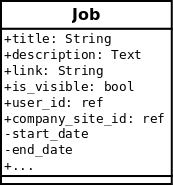
\includegraphics[width=0.3\textwidth]{./diagrams/job-erm.png}
 % job-erm.png: 173x186 pixel, 51dpi, 8.65x9.30 cm, bb=0 0 245 264
 \caption{Attribute des Modells "`Job"'}
  \label{fig:job-erm}
\end{figure}

Während der Analyse wurden die benötigten Attribute bestimmt. In Abbildung \ref{fig:job-erm} sei z.B. ein Fragment des Grobdesigns, in dem die Basisattribute der Tabelle dargestellt werden. Neben den einfachen Attributen, wie Title, Description und Link, existieren auch Referenzen auf andere Objekte (d.h. dies stellen Fremdschlüssel zu anderen Tabellen dar), wie z.B. Schlagwörter (Tags), ein Besitzer einer Stellenanzeige (User) und so weiter.

Einer der häufigsten Wege, ein Modell und dessen Datenbankschema zu generieren, ist die Nutzung des mitgelieferten Codegenerators. Mittels des Kommandos:

\shadebox{  
  rails generate model MODELLNAME spalte1:datentyp1 spalte2:datentyp2 ...
}

generieren wird ein Modell mit dem angegebenen Modellnamen. Dazu geben wir paarweise die gewünschten Spaltennamen und deren Datentypen an (string, text, datetime, references, integer, boolean, decimal, ...).
\begin{lstlisting}
~/it-jobs$ rails generate model job title:string link:string \
    description:text user:references visible:boolean ...

      invoke  active_record
      create    db/migrate/20110828160636_create_jobs.rb
      create    app/models/job.rb
      invoke    test_unit
      create      test/unit/job_test.rb
      create      test/fixtures/jobs.yml

\end{lstlisting}
Mit der Anweisung uns ein Modell "'job"` mit den nachfolgenden Attributen zu generieren, hat Rails uns nun schon ein Stück Arbeit abgenommen. 

Es wurden erstellt:
\begin{itemize}
 \item Eine Migration (\verb|db/migrate/2011xxxxxx_create_jobs.rb|). Dies stellt eine datenbankunabhängige Repräsentation einer Änderung an der Struktur unserer Datenbank dar. In diesem ist es die Erstellung einer Tabelle "'jobs"` (beachte: Plural!), mit den Spalten Titel, Link als String, Description als Textfeld, eine User\_ID als Referenz auf ein anderes Modell usw.
 \item Die Modelklasse (\verb|app/models/job.rb|). Trotz unserer Definition der Spalten und deren Typen über die Kommandozeile, ist diese Klasse leer. Da wir ActiveRecord verwenden, definieren wir die Attribute, die unser Modell hat, nicht in der Modellklasse, sondern ausschließ in der Datenbank. Die Migration erspart uns die manuelle Arbeit, selbst in unserer Datenbank Spalten anzulegen. Bei Initialisierung eines Modells lädt ActiveRecord die Spalteninformationen aus der Datenbank, und generiert dafür Getter und Setter Methoden. 
 \item Die dazugehörige Testklasse (\verb|app/unit/job_test.rb|)
 \item und Fixtures-Datei (\verb|test/fixtures/jobs.yml|), zur Definition von Testdaten. 
\end{itemize}

Die Migration liegt nun zwar vor, aber es existiert noch keine Datenbank und demnach auch noch keine Tabelle mit dem Namen "`jobs"'. Dazu weisen wir nun Rails an, alle offenen Migrationen auszuführen. Standardmäßig erstellt Rails dann selbstständig eine SQLite Datenbank unter "`db/development.sqlite3"'.
Danach können wir die Rails-Test-Suite auch schon ausführen:

\begin{lstlisting}
$ rake db:migrate && rake test
 
==  CreateJobs: migrating =========================
-- create_table(:jobs)
   -> 0.0020s
==  CreateJobs: migrated (0.0021s) ================

(in /home/zealot64/TEST)
Loaded suite /usr/lib/ruby/gems/1.8/gems/rake-0.8.7/lib/rake/rake_test_loader
Started
.
Finished in 0.043818 seconds.

1 tests, 1 assertions, 0 failures, 0 errors

\end{lstlisting}

Es wurde also schon ein Testfall erfolgreich ausgeführt, nämlich ein Dummytestfall von Rails:

\begin{ruby}[label={test/units/job\_test.rb}]
\PY{c+c1}{#test/unit/job\PYZus{}test.rb }
\PY{n+nb}{require} \PY{l+s+s1}{'test\PYZus{}helper'}

\PY{k}{class} \PY{n+nc}{JobTest} \PY{o}{<} \PY{n+no}{ActiveSupport}\PY{o}{::}\PY{n+no}{TestCase}
  \PY{c+c1}{# Replace this with your real tests.}
  \PY{n+nb}{test} \PY{l+s+s2}{"}\PY{l+s+s2}{the truth}\PY{l+s+s2}{"} \PY{k}{do}
    \PY{n}{assert} \PY{k+kp}{true}
  \PY{k}{end}
\PY{k}{end}
\end{ruby}
\label{list:bla}
\captionsetup{type=lstlisting}
\caption{Listing Test}


\paragraph{2. Testen auf Validierung}

Ein Feature von Rails umfassen die sogenannten Validierungen. Diese stellen sicher, dass eine Instanz eines Modells nur dann gespeichert ist, wenn es gewissen Kritieren entspricht. Viele der Validations sind vergleichbar mit den Datenbank-Constraints einiger Datenbanken. Rails nutzt diese standardmäßig nicht, da es auch andere Persistenzsysteme unterstützt, wie z.B. Key-Value-Store oder sogenannte NoSQL Datenbanken. So stellt Rails die Konsistenz und referenzielle Integrität innerhalb der Applikationsschicht sicher.

Nun möchten wir sicherstellen, dass eine Stellenanzeige nur dann gespeichert wird, wenn sie einen Titel beinhaltet. Der Test dazu würde wie folgt lauten:

\begin{ruby}[label={test/units/job\_test.rb}]
\PY{n+nb}{require} \PY{l+s+s1}{'test\PYZus{}helper'}

\PY{k}{class} \PY{n+nc}{JobTest} \PY{o}{<} \PY{n+no}{ActiveSupport}\PY{o}{::}\PY{n+no}{TestCase}
  \PY{n+nb}{test} \PY{l+s+s2}{"}\PY{l+s+s2}{ein Job muss einen Titel haben}\PY{l+s+s2}{"} \PY{k}{do}
    \PY{n}{job} \PY{o}{=} \PY{n+no}{Job}\PY{o}{.}\PY{n}{new}
    \PY{n}{job}\PY{o}{.}\PY{n}{title} \PY{o}{=} \PY{k+kp}{nil}
    \PY{n}{assert} \PY{o}{!}\PY{n}{job}\PY{o}{.}\PY{n}{save}
  \PY{k}{end}
\PY{k}{end}
\end{ruby}
\codecaption{Test auf Vorhandensein eines Titels}
\tddred
Zuerst instanziieren wir einen Job, und geben ihm explizit einen leeren Titel, um das Testziel nochmal herauszustellen. Danach rufen wir die "`save"'-Methode auf, die prüft, ob alle Validierungskritierien erfolgt sind, und speichert das Objekt persistent in der Datenbank im Erfolgsfall. Dann gibt "`save"' ein "`true"' zurück, anderfalls, d.h. wenn die Validierung fehlschlug, "`false"'.
Der Ablauf ist in der Abbildung \ref{fig:activerecordsave} noch einmal erläutert.

\begin{figure}[hbp]
 \centering
 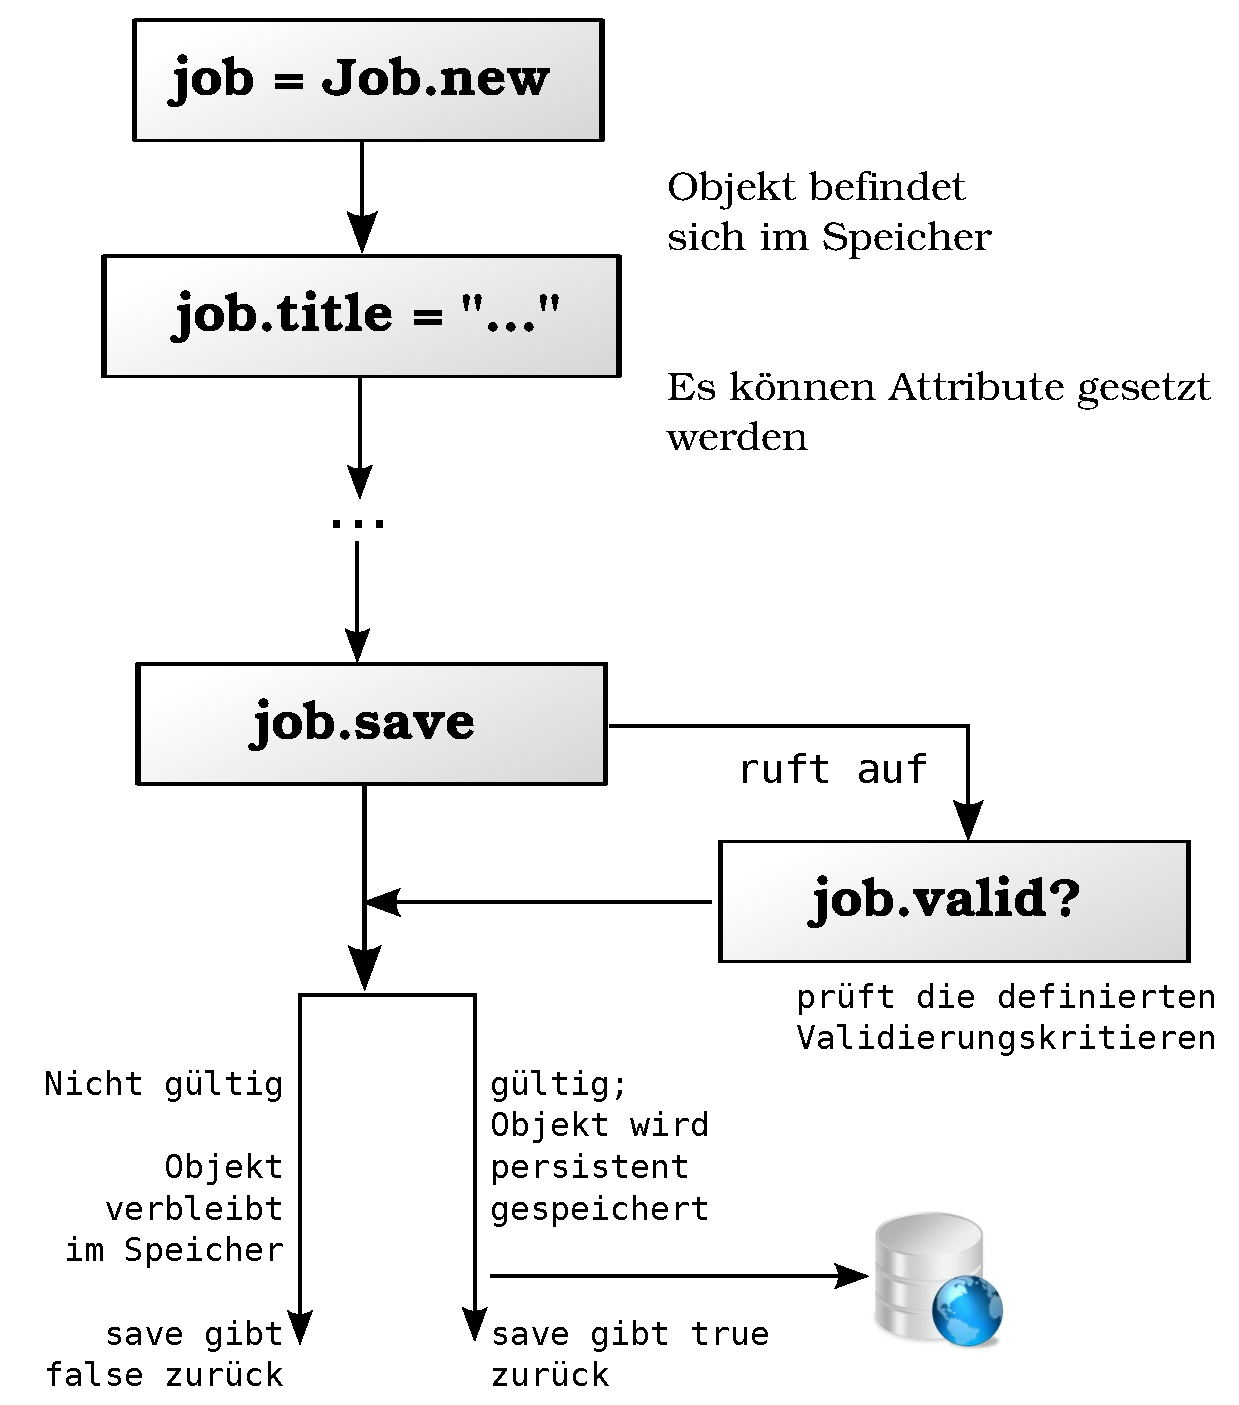
\includegraphics[width=0.8\textwidth]{./diagrams/activerecord-save.pdf}
 % activerecord-save.pdf: 595x675 pixel, 72dpi, 20.99x23.81 cm, bb=0 0 595 675
 \caption{Funktionsweise von save bei ActiveRecord Objekten}
 \label{fig:activerecordsave}
\end{figure}

Da wir noch keine Validierungskritieren implementiert haben, schlägt dieser Test fehl, da das Objekt gespeichert wurde.

Unser nächstes Ziel ist es nun, mit so wenig Code wie möglich den Test bestehen zu lassen. Das können wir mittels der eingebauten wie schon erwähnten Validierungen:

\begin{ruby}[label=app/models/job.rb]
\PY{k}{class} \PY{n+nc}{Job} \PY{o}{<} \PY{n+no}{ActiveRecord}\PY{o}{::}\PY{n+no}{Base}
  \PY{n}{validates} \PY{l+s+ss}{:title}\PY{p}{,} \PY{l+s+ss}{:presence} \PY{o}{=}\PY{o}{>} \PY{k+kp}{true}
\PY{k}{end}
\end{ruby}
\codecaption{Implementierung der Validierung in die Klasse Job}
"`validates"' ist eine Funktion aus der ActiveRecord Bibliothek, die zwei Parameter entgegennimmt: Der erste ist die Spalte, auf der sich die Validierung bezieht, als Zweites folgt eine Liste an Validierungskritieren. Hier ist das Kritierum "`presence"', also das Vorhandensein eines nicht-leeren Attributs. Weitere Kritieren sind z.B. Format, Länge, Minimum, Maximum, oder selbst definierte Kriterien.

\tddgreen
Nach erneuter Ausführung der Testsuite, besteht der Test nun. Jetzt folgt die Refaktorisierungsphase. Der Programmcode lässt sich nicht weiter vereinfachen. Aber der Testcode ist ausdrücklich nicht von Refaktorisierungen befreit, und eine Refaktorisierung wäre z.B.:
\tddrefactor
\begin{ruby}[label=test/unit/job\_test.rb]
\PY{n+nb}{test} \PY{l+s+s2}{"}\PY{l+s+s2}{ein Job muss einen Titel haben}\PY{l+s+s2}{"} \PY{k}{do}
  \PY{n}{job} \PY{o}{=} \PY{n+no}{Job}\PY{o}{.}\PY{n}{new} \PY{l+s+ss}{:title} \PY{o}{=}\PY{o}{>} \PY{k+kp}{nil}
  \PY{n}{assert} \PY{o}{!}\PY{n}{job}\PY{o}{.}\PY{n}{save}
\PY{k}{end}
\end{ruby}
\codecaption{refaktorisierter Test}

Nun wollen wir dasselbe für das Feld E-Mail tun, hierbei aber nicht nur das Vorhandensein prüfen, sondern auch das Format.

\begin{ruby}[label=test/unit/job\_test.rb]
\PY{n+nb}{test} \PY{l+s+s2}{"}\PY{l+s+s2}{ein Job muss eine gültige E-Mail haben}\PY{l+s+s2}{"} \PY{k}{do}
  \PY{n}{job} \PY{o}{=} \PY{n+no}{Job}\PY{o}{.}\PY{n}{new} \PY{l+s+ss}{:email} \PY{o}{=}\PY{o}{>} \PY{l+s+s2}{"}\PY{l+s+s2}{invalid\PYZus{}email}\PY{l+s+s2}{"}
  \PY{n}{assert} \PY{o}{!}\PY{n}{job}\PY{o}{.}\PY{n}{save}
\PY{k}{end}
\end{ruby}
\tddred
Die Implementierung wäre dann:
\begin{ruby}[label=app/models/job.rb]
\PY{k}{class} \PY{n+nc}{Job} \PY{o}{<} \PY{n+no}{ActiveRecord}\PY{o}{::}\PY{n+no}{Base}
  \PY{n}{validates} \PY{l+s+ss}{:email}\PY{p}{,} \PY{l+s+ss}{:format} \PY{o}{=}\PY{o}{>} \PY{l+s+sr}{/}\PY{l+s+sr}{\PYZca{}[}\PY{l+s+sr}{\PYZbs{}}\PY{l+s+sr}{w}\PY{l+s+sr}{\PYZbs{}}\PY{l+s+sr}{d\PYZus{}}\PY{l+s+sr}{\PYZbs{}}\PY{l+s+sr}{-]+@[}\PY{l+s+sr}{\PYZbs{}}\PY{l+s+sr}{w}\PY{l+s+sr}{\PYZbs{}}\PY{l+s+sr}{d\PYZus{}}\PY{l+s+sr}{\PYZbs{}}\PY{l+s+sr}{-]}\PY{l+s+sr}{\PYZbs{}}\PY{l+s+sr}{.[}\PY{l+s+sr}{\PYZbs{}}\PY{l+s+sr}{w}\PY{l+s+sr}{\PYZbs{}}\PY{l+s+sr}{d]\PYZob{}2,3\PYZcb{}\$}\PY{l+s+sr}{/}
  \PY{o}{.}\PY{n}{.}\PY{o}{.}
\PY{k}{end}
\end{ruby}
\tddgreen
Eine Refaktorisierung ist aufgrund der Einfachheit der Beispiel hier nur gering möglich. Man könnte z.B. den regulären Ausdruck, der das Format der E-Mail Adresse beschreibt in eine neue Klasse oder zumindest eine Konstante auslagern. Wir wählen eine Konstante, die beim Laden von Rails bereitgestellt wird.
\tddrefactor
\begin{ruby}[label=config/initializers/job.rb und app/models/job.rb]
\PY{c+c1}{# config/initializers/regex.rb}
\PY{n+no}{REGEX\PYZus{}EMAIL\PYZus{}FORMAT} \PY{o}{=} \PY{l+s+sr}{/}\PY{l+s+sr}{\PYZca{}[}\PY{l+s+sr}{\PYZbs{}}\PY{l+s+sr}{w}\PY{l+s+sr}{\PYZbs{}}\PY{l+s+sr}{d\PYZus{}}\PY{l+s+sr}{\PYZbs{}}\PY{l+s+sr}{-]+@[}\PY{l+s+sr}{\PYZbs{}}\PY{l+s+sr}{w}\PY{l+s+sr}{\PYZbs{}}\PY{l+s+sr}{d\PYZus{}}\PY{l+s+sr}{\PYZbs{}}\PY{l+s+sr}{-]}\PY{l+s+sr}{\PYZbs{}}\PY{l+s+sr}{.[}\PY{l+s+sr}{\PYZbs{}}\PY{l+s+sr}{w}\PY{l+s+sr}{\PYZbs{}}\PY{l+s+sr}{d]\PYZob{}2,3\PYZcb{}\$}\PY{l+s+sr}{/}

\PY{c+c1}{# app/models/job.rb}
\PY{k}{class} \PY{n+nc}{Job} \PY{o}{<} \PY{n+no}{ActiveRecord}\PY{o}{::}\PY{n+no}{Base}
  \PY{n}{validates} \PY{l+s+ss}{:email}\PY{p}{,} \PY{l+s+ss}{:format} \PY{o}{=}\PY{o}{>} \PY{n+no}{REGEX\PYZus{}EMAIL\PYZus{}FORMAT}
    \PY{o}{.}\PY{n}{.}\PY{o}{.}
\PY{k}{end}
\end{ruby}
\codecaption{Auslagerung des Regulären Ausdrucks in einen Initalisierer}
Ein erneutes Ausführen der Tests betätigt den Erfolg der Refaktorisierung.

\paragraph{3. Refaktorisierungen der Testklasse}
Nun fehlt aber noch die Definition eines Positiv-Beispiel für einen gültigen Job.

\begin{ruby}[label=test/unit/job\_test.rb]
...
\PY{n+nb}{test} \PY{l+s+s2}{"}\PY{l+s+s2}{ein vollstaendiger Job muss gueltig seinn}\PY{l+s+s2}{"} \PY{k}{do}
  \PY{n}{job} \PY{o}{=} \PY{n+no}{Job}\PY{o}{.}\PY{n}{new} \PY{l+s+ss}{:title} \PY{o}{=}\PY{o}{>} \PY{l+s+s2}{"}\PY{l+s+s2}{Rails Entwickler}\PY{l+s+s2}{"}\PY{p}{,} \PY{l+s+ss}{:email} \PY{o}{=}\PY{o}{>} \PY{l+s+s2}{"}\PY{l+s+s2}{info@stefanwienert.net}\PY{l+s+s2}{"}
  \PY{n}{assert\PYZus{}valid} \PY{n}{job}
\PY{k}{end}
\end{ruby}
\tddgreen
Dieser Test besteht sofort, macht also genau genommen keine weitere Aussage über unser System. Nach der "`reinen"' Testgetriebenen Leere sollte dieser entfernt werden. Es ist allerdings eine gute Strategie, bei Validierungen mindestens ein Beispiel zu präsentieren, dass angenommen wird. Nichtsdestotrotz können wir nun Refaktorisieren. Insbesondere unsere Testfunktionen enthalten unnötige Redundanzien:

\begin{ruby}[label=test/unit/job\_test.rb]
\PY{n+nb}{test} \PY{l+s+s2}{"}\PY{l+s+s2}{ein Job muss einen Titel haben}\PY{l+s+s2}{"} \PY{k}{do}
  \PY{n}{job} \PY{o}{=} \PY{n+no}{Job}\PY{o}{.}\PY{n}{new} \PY{l+s+ss}{:title} \PY{o}{=}\PY{o}{>} \PY{k+kp}{nil}
  \PY{n}{assert} \PY{o}{!}\PY{n}{job}\PY{o}{.}\PY{n}{save}
\PY{k}{end}
\PY{n+nb}{test} \PY{l+s+s2}{"}\PY{l+s+s2}{ein Job muss eine gültige E-Mail haben}\PY{l+s+s2}{"} \PY{k}{do}
  \PY{n}{job} \PY{o}{=} \PY{n+no}{Job}\PY{o}{.}\PY{n}{new} \PY{l+s+ss}{:email} \PY{o}{=}\PY{o}{>} \PY{l+s+s2}{"}\PY{l+s+s2}{invalid\PYZus{}email}\PY{l+s+s2}{"}
  \PY{n}{assert} \PY{o}{!}\PY{n}{job}\PY{o}{.}\PY{n}{save}
\PY{k}{end}
\PY{n+nb}{test} \PY{l+s+s2}{"}\PY{l+s+s2}{ein vollstaendiger Job muss gueltig seinn}\PY{l+s+s2}{"} \PY{k}{do}
  \PY{n}{job} \PY{o}{=} \PY{n+no}{Job}\PY{o}{.}\PY{n}{new} \PY{l+s+ss}{:title} \PY{o}{=}\PY{o}{>} \PY{l+s+s2}{"}\PY{l+s+s2}{Rails Entwickler}\PY{l+s+s2}{"}\PY{p}{,} \PY{l+s+ss}{:email} \PY{o}{=}\PY{o}{>} \PY{l+s+s2}{"}\PY{l+s+s2}{info@stefanwienert.net}\PY{l+s+s2}{"}
  \PY{n}{assert\PYZus{}valid} \PY{n}{job}
\PY{k}{end}
\end{ruby}
\codecaption{Alle bisherigen Testmethoden in der Klasse JobTest}
\tddrefactor
In allen drei Methoden wird ein Job instanziiert, und lediglich verschiedene Attribute überprüft. Auch haben unsere ersten beiden Tests keine gültige Aussage mehr, da der jeweilige Job sowieso nicht gültig ist, da jeweils das andere Attribut fehlt\footnote{Im ersten Test ist nicht nur der Titel nicht gesetzt, sondern auch die E-Mail entspricht nicht dem Format}. Es ist also höchste Zeit, die Tests zu refaktorisieren. Dies geschieht am Besten durch die Verwendung einer Testdaten-Generation, z.B. den eingebauten Fixtures, die Rails uns bei der Codegeneration schon mit generiert hatte. Dabei definieren wir zentralisiert unsere (gültigen) Testdaten, die von Rails vor jedem einzelnen Test in der Datenbank bereitgestellt werden:

\begin{ruby}[label=test/fixtures/jobs.yml]
\PY{l+lScalar+lScalarPlain}{valid\PYZus{}job}\PY{p+pIndicator}{:}
  \PY{l+lScalar+lScalarPlain}{title}\PY{p+pIndicator}{:} \PY{l+lScalar+lScalarPlain}{Rails}\PY{l+lScalar+lScalarPlain}{ }\PY{l+lScalar+lScalarPlain}{Entwickler}
  \PY{l+lScalar+lScalarPlain}{email}\PY{p+pIndicator}{:} \PY{l+lScalar+lScalarPlain}{info@stefanwienert.net}
  \PY{l+lScalar+lScalarPlain}{link}\PY{p+pIndicator}{:} \PY{l+s}{"}\PY{l+s}{http://www.example.com/jobs}\PY{l+s}{"}
  \PY{l+lScalar+lScalarPlain}{visible}\PY{p+pIndicator}{:} \PY{l+lScalar+lScalarPlain}{true}
  \PY{l+lScalar+lScalarPlain}{...}
\PY{l+lScalar+lScalarPlain}{invisible\PYZus{}job}\PY{p+pIndicator}{:}
  \PY{l+lScalar+lScalarPlain}{title}\PY{p+pIndicator}{:} \PY{l+lScalar+lScalarPlain}{Rails}\PY{l+lScalar+lScalarPlain}{ }\PY{l+lScalar+lScalarPlain}{Entwickler}
  \PY{l+lScalar+lScalarPlain}{visible}\PY{p+pIndicator}{:} \PY{l+lScalar+lScalarPlain}{false}
  \PY{l+lScalar+lScalarPlain}{...}
\end{ruby}
\codecaption{Fixtures Testdaten für zwei Jobs}

Nun können wir diese Fixtures in unseren Tests verwenden, und das ganze in einer setup-Methode, die vor jedem Testfall aufgerufen wird, laden:
\tddrefactor
\begin{ruby}[label=test/unit/job\_test.rb]
\PY{k}{class} \PY{n+nc}{JobTest} \PY{o}{<} \PY{n+no}{ActiveSupport}\PY{o}{::}\PY{n+no}{TestCase}
  \PY{n}{setup} \PY{k}{do}
    \PY{n+nv+vi}{@job} \PY{o}{=} \PY{n}{jobs} \PY{l+s+ss}{:valid\PYZus{}job}
    \PY{c+c1}{# Dies lädt den Job mit dem Schlüssel "valid\PYZus{}job" und schreibt ihn }
    \PY{c+c1}{#  in die Instanzvariable @job der Testklasse}
  \PY{k}{end}
  \PY{n+nb}{test} \PY{l+s+s2}{"}\PY{l+s+s2}{stelle sicher, dass die Fixtures valide sind}\PY{l+s+s2}{"} \PY{k}{do}
    \PY{n}{assert\PYZus{}valid} \PY{n+nv+vi}{@job}
  \PY{k}{end}
  \PY{n+nb}{test} \PY{l+s+s2}{"}\PY{l+s+s2}{ein Job muss einen Titel haben}\PY{l+s+s2}{"} \PY{k}{do}
    \PY{n+nv+vi}{@job}\PY{o}{.}\PY{n}{title} \PY{o}{=} \PY{k+kp}{nil}
    \PY{n}{assert} \PY{o}{!}\PY{n+nv+vi}{@job}\PY{o}{.}\PY{n}{save}
  \PY{k}{end}
  \PY{n+nb}{test} \PY{l+s+s2}{"}\PY{l+s+s2}{ein Job muss eine gültige E-Mail haben}\PY{l+s+s2}{"} \PY{k}{do}
    \PY{n+nv+vi}{@job}\PY{o}{.}\PY{n}{email} \PY{o}{=} \PY{l+s+s2}{"}\PY{l+s+s2}{invalid\PYZus{}email}\PY{l+s+s2}{"}
    \PY{n}{assert} \PY{o}{!}\PY{n+nv+vi}{@job}\PY{o}{.}\PY{n}{save}
  \PY{k}{end}
\PY{k}{end}
\end{ruby}
\codecaption{Finale Job-Test Klasse nach Refaktorisierung}



Am Ende dieser Refaktorisierungen ist es notwendig, die Tests noch einmal auszuführen.
\tddgreen
Danach würde die Implementierung einer nächsten Teilanforderung sein. 

In diesem Abschnitt war zu sehen, dass die Testgetriebene Entwicklung das Arbeiten und Testen in kleinen Schritten favorisiert.
